\section{Introduction}
\looseness=-1
\begin{figure*}[!htb]
    \centering
    % \vspace{-25pt}
    % 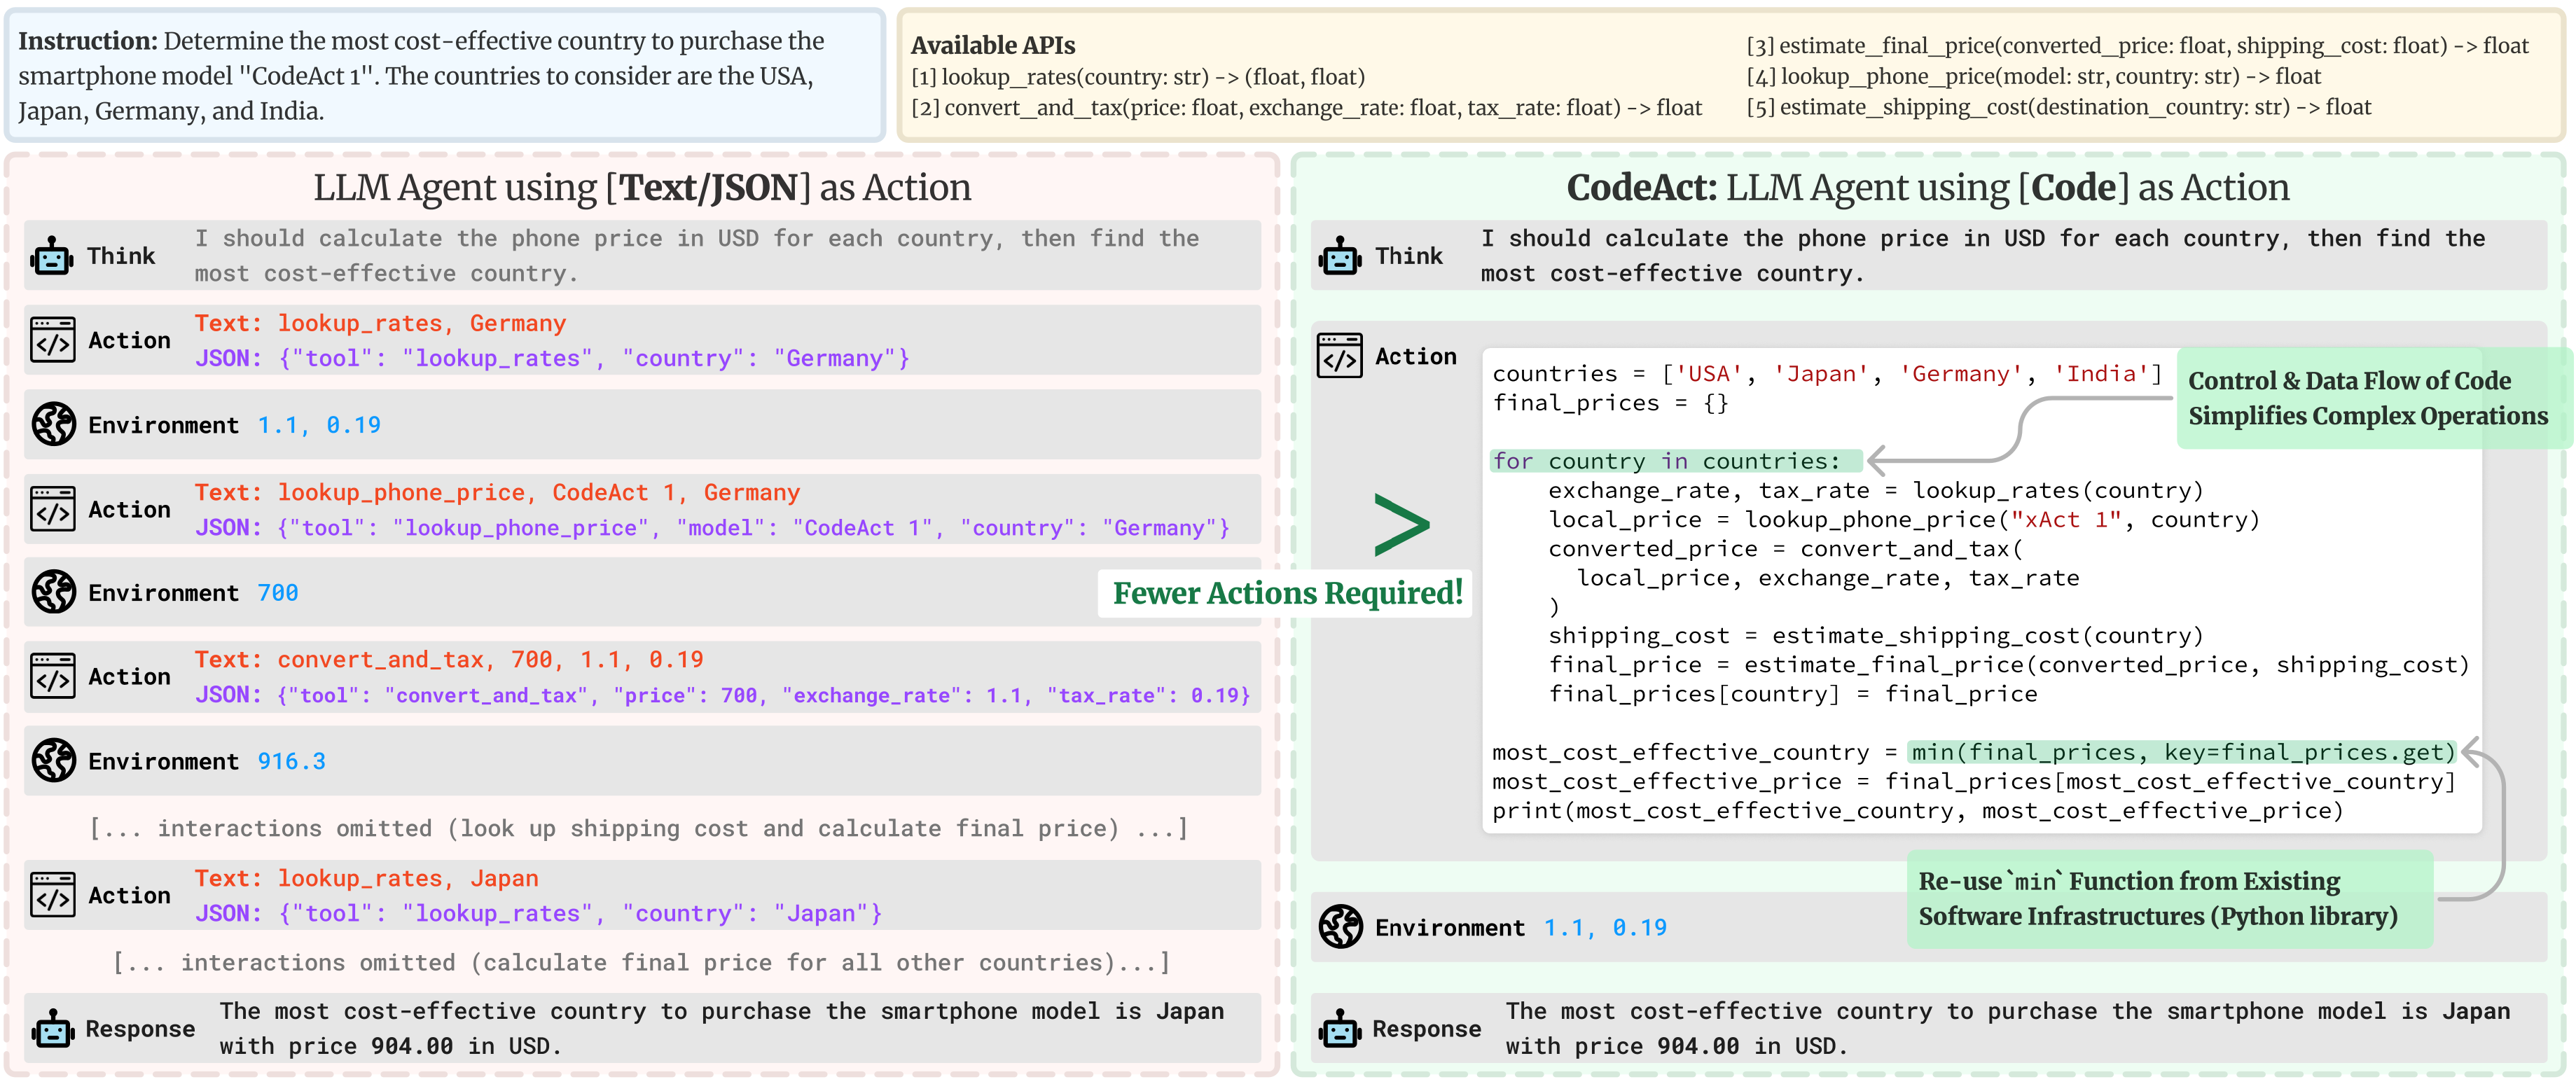
\includegraphics[width=0.9\textwidth]{figures/code_vs_text_json_compare.pdf}
    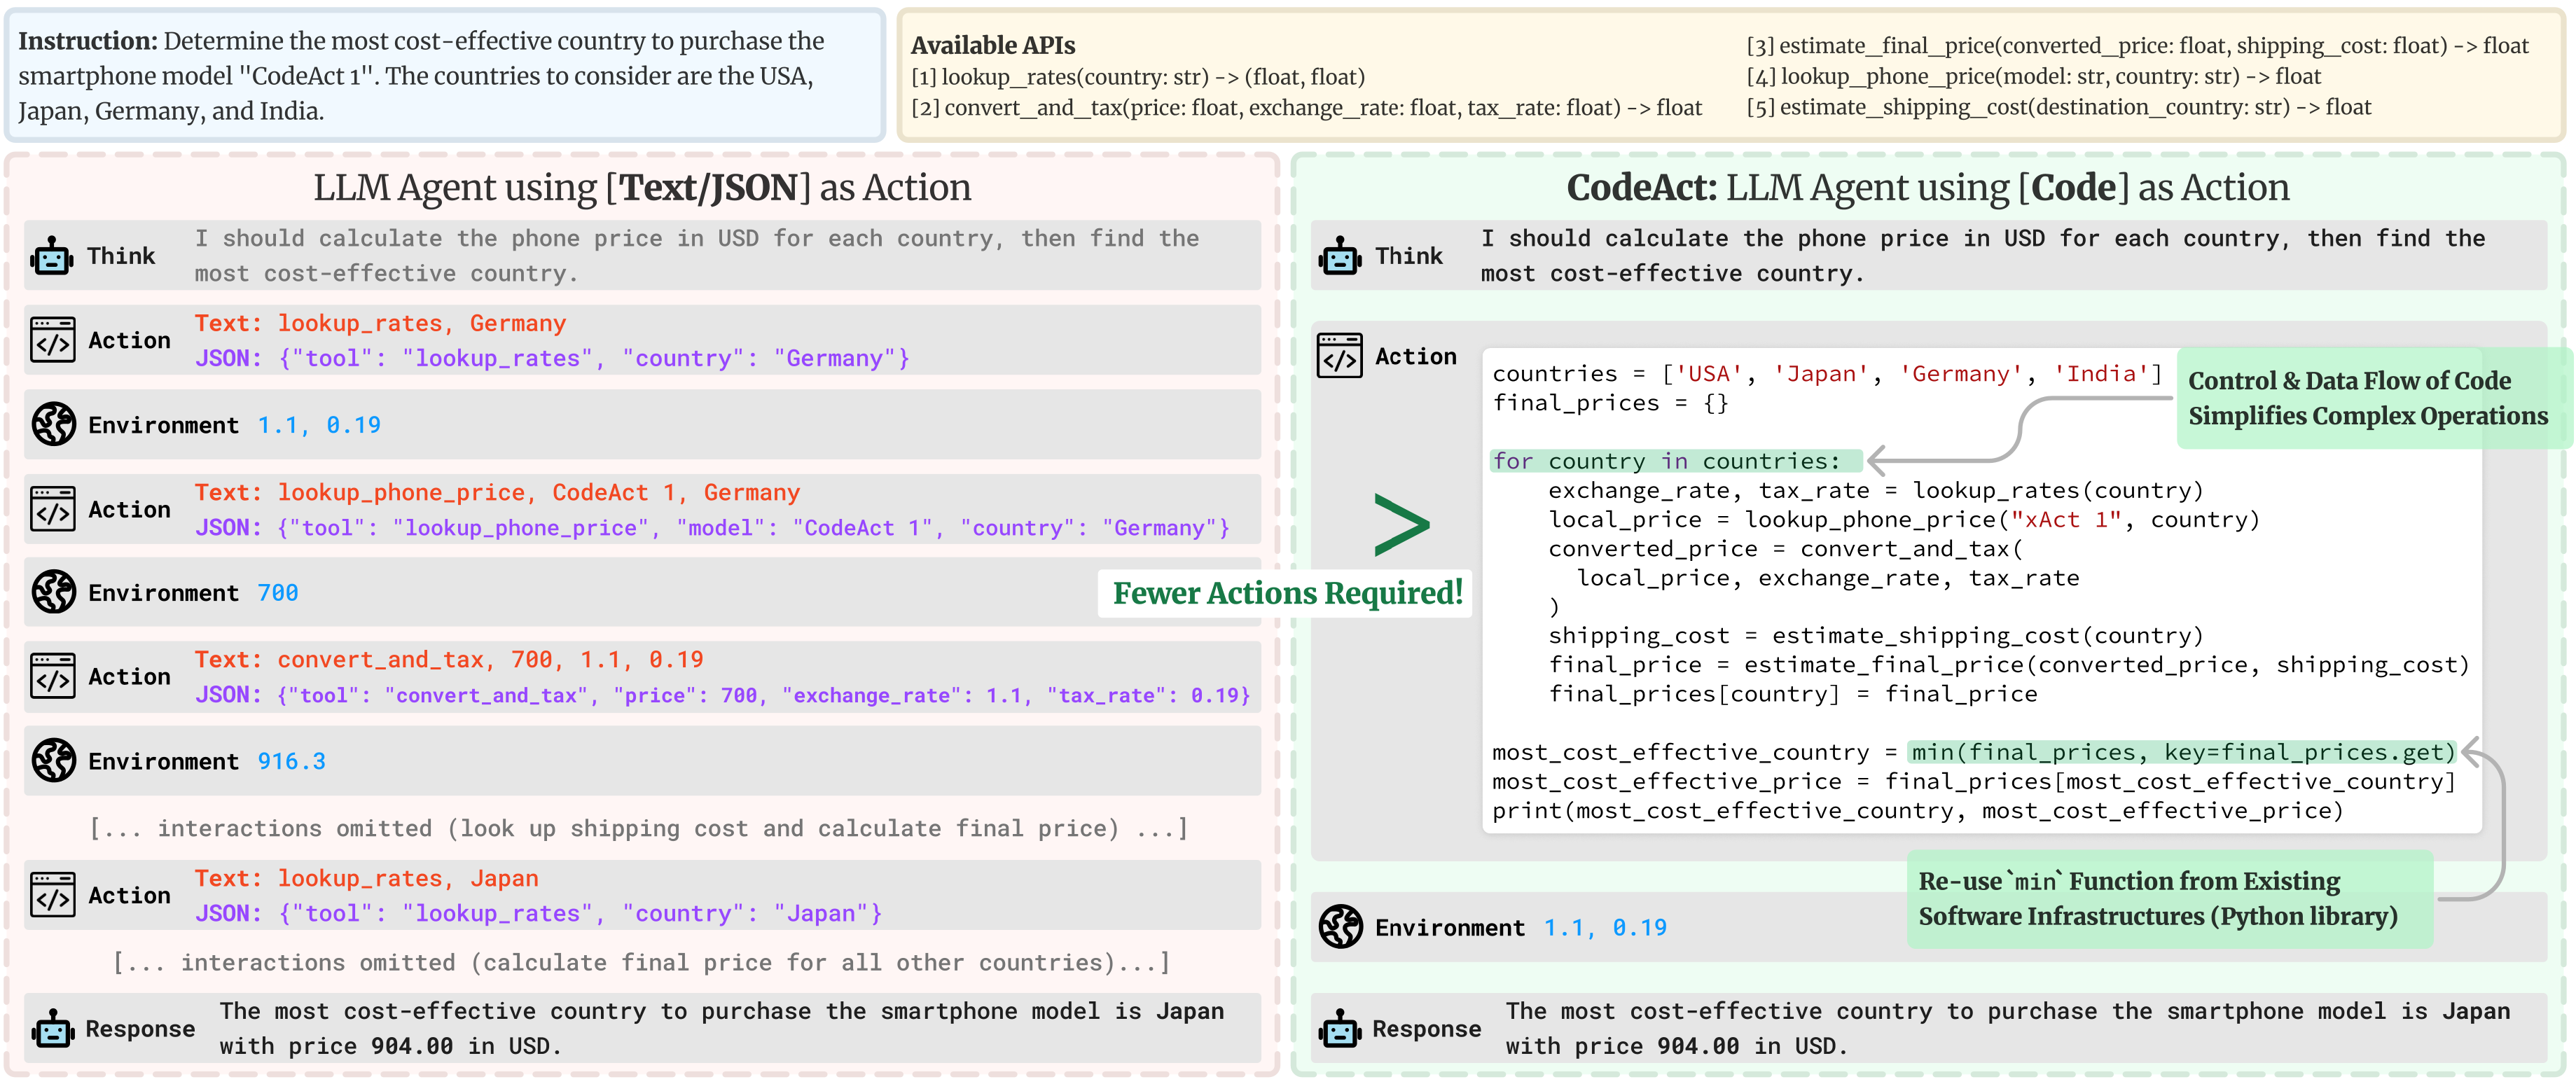
\includegraphics[width=\textwidth]{figures/code_vs_text_json_compare.pdf}
    % \vspace{-3mm}
    % ---------
    % \vspace{2mm}
    \vspace{-5pt}
    % ---------
    % 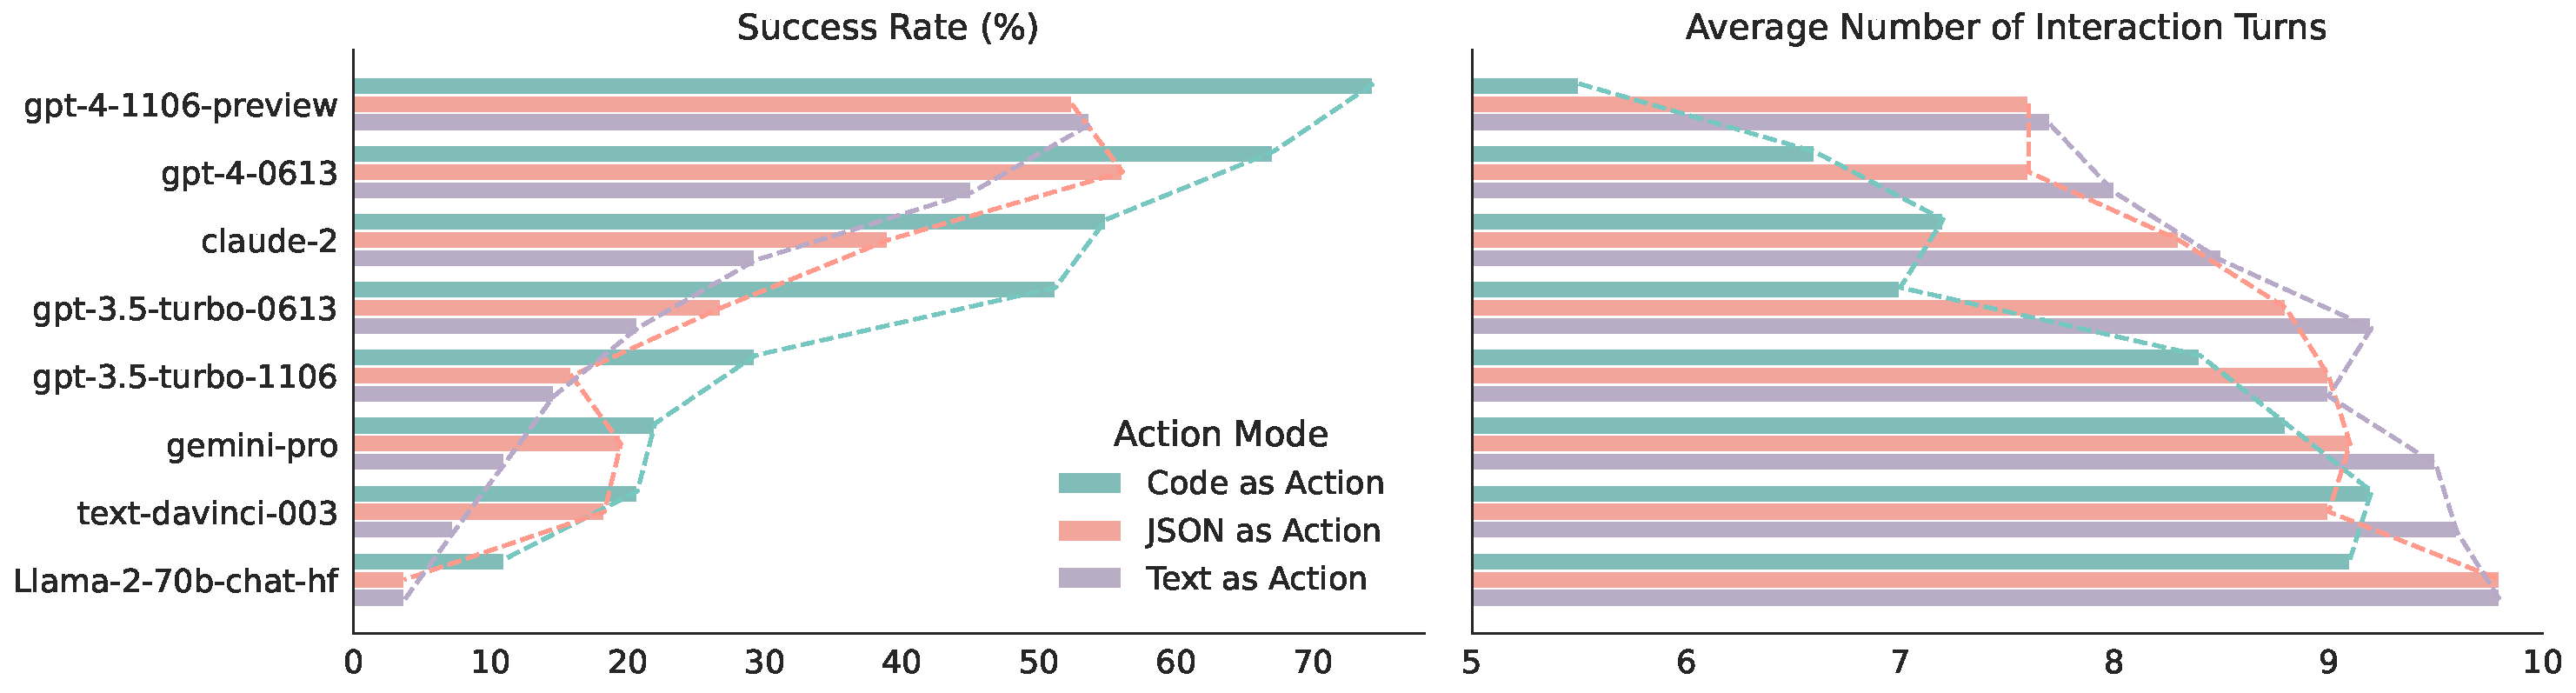
\includegraphics[width=0.9\textwidth]{figures/zeroshot_act_model_performance.pdf}
    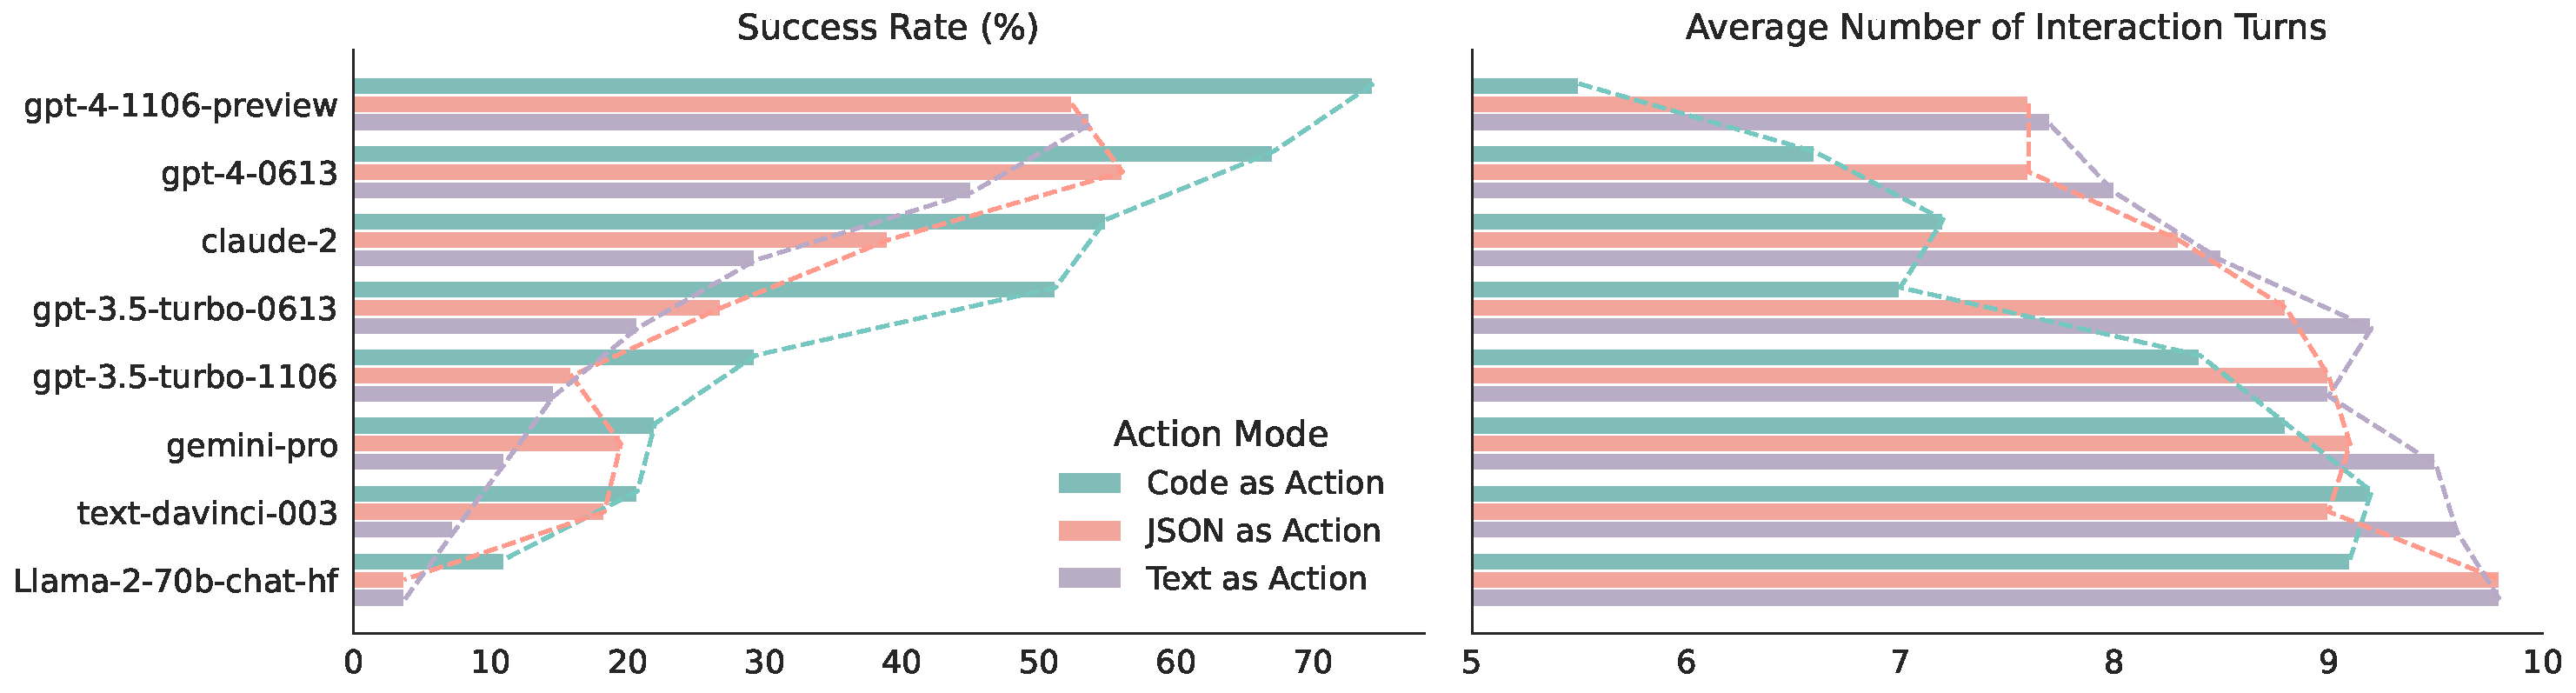
\includegraphics[width=\textwidth]{figures/zeroshot_act_model_performance.pdf}
    \vspace{-15pt}
    \caption{Comparison between \approach and Text / JSON as action. \textbf{(top)} Illustrative example comparing different actions. \textbf{(bottom)} Quantitative results on \evalname (\sref{sec:control-data-flow}).}
    \label{fig:illustrative_example}
    \label{fig:zeroshot_acteval} 
    % \vspace{-18pt}
\end{figure*}


Large Language Models (LLMs) have emerged as a pivotal breakthrough in natural language processing (NLP).
% 
When augmented with \textit{action} modules that allow access to APIs, their action space expands beyond conventional text processing, allowing LLMs to acquire capabilities such as tool invocation and memory management~\citep{mialon2023augmented, schick2023toolformer} and venture into real-world tasks such as controlling robots~\citep{saycan2022arxiv,huang2023voxposer,ma2023eureka} and performing scientific experiments~\citep{bran2023chemcrow}.

We inquire: \textit{how to effectively expand LLM agents' action space for solving complex real-world problems?} 
Much existing research has examined using text~\interalia{yao2022react,park2023generative} or JSON~\interalia{Qin2023ToolLLMFL,Chase_LangChain_2022} to produce actions (e.g., tool uses in \fref{fig:illustrative_example} top left).
% 
However, both methods typically suffer from constrained scope of action spaces (actions are usually tailored for specific tasks) and restricted flexibility (e.g., inability to compose multiple tools in a single action).
% 
As an alternative approach, several work \citep{codeaspolicies2022,progprompt,wang2023voyager} demonstrate the potential of using LLMs to generate code to control robots or game characters.
However, they typically rely on pre-specified control primitives and hand-engineered prompts and, more importantly, struggle to dynamically adjust or emit actions based on new environmental observation and feedback.

This work proposes \approach, a general-purpose framework that allows LLMs to generate executable Python \textbf{code} as \textbf{act}ions (\fref{fig:illustrative_example} top right).
% 
\approach is designed to handle a variety of applications and comes with unique advantages:
% 
% \begin{itemize}[noitemsep,topsep=0pt,parsep=0pt,partopsep=0pt]
\begin{itemize}[noitemsep,topsep=0pt,parsep=0pt,partopsep=0pt,leftmargin=18pt]
\item[(1) ]Integrated with a Python interpreter, \approach can execute code actions and \textit{dynamically adjust prior actions or emit new action} based on observations (e.g., code execution results) it receives through multiple turns of interactions.

\item[(2)]
Code actions allow LLM to leverage existing \textit{software packages}. \approach can use readily available Python packages for an expanded action space instead of hand-crafted task-specific tools \citep{Yuan2023CRAFTCL,shen2023hugginggpt}. It also allows LLM to use automated feedback (e.g., error messages) implemented in most software to improve task-solving by self-debugging its generated code \citep{chen2023teaching,Wang2023LeTI}.

\item[(3)] 
\textit{Code data} is widely used in pre-training today's  LLMs \citep{yang2024llm}.
These models are already familiar with structured programming languages, allowing cost-effective adoption of \approach.

\item[(4)]
Compared to JSON and text with a pre-defined format, code inherently supports \textit{control and data flow}, allowing for the storage of intermediate results as variables for reuse and the composition of multiple tools to perform complex logical operations (e.g., if-statements, for-loops) with \textit{one} piece of code, thereby unlocking LLMs' potential to tackle complex tasks by leveraging its pre-trained knowledge of programming.
% 
In \fref{fig:illustrative_example}, an LLM using with \approach (top right) can apply the same sequence of tools (e.g., passing one tool's output as input to another tool using the data flow feature) to \textit{all} inputs through for-loops (i.e., control flow feature) with \textit{one} action; while text or JSON have to take action for every input (top left).
\end{itemize}

Our extensive experiments with 17 LLMs (including both open-source and proprietary ones) confirm the above benefits (3 
\& 4) of \approach.
% 
To demonstrate benefit (3), our first experiment (\sref{sec:data-factor-format}) compares \approach to baselines on basic tasks involving \textit{atomic tool use} (i.e., only one tool is used per action), ablating the control and data flow advantage offered by \approach.
The results show that, for most LLMs, \approach achieves comparable or better performance than the baselines.
% 
\approach's performance gains are more prominent on complex tasks, as demonstrated in our second experiment (benefit 4).
We curate a new benchmark consisting of 82 human-curated tasks that typically require \textbf{m}ultiple calls to \textbf{m}ultiple tools in \textbf{m}ulti-turn interactions (\evalname; \sref{sec:control-data-flow}).
Problems in this benchmark often require intricate coordination and composition of multiple tools.
% 
With its strengths in control and data flow, \approach achieves up to a 20\% absolute improvement over baselines on the success rate of solving the problems while requiring up to 30\% fewer actions.
% 
These performance gains widen as the capabilities of the LLMs increase (\fref{fig:illustrative_example} bottom).

The promising performance of \approach motivates an open-source LLM agent that can effectively act through \approach, and collaborate with humans through natural language.
% 
To this end, we collect an instruction-tuning dataset \dataname consisting of 7k high-quality multi-turn interaction trajectories with \approach (\sref{sec:agent_env_data}).
% 
\dataname is motivated by a general agent framework consisting of agent, user, and environments (\fref{fig:llm_agent_framework}) and focuses on agent-environment interactions with the computer (information seeking, software package use, external memory) and the physical world (robot planning).
% 
On \dataname, we perform careful data selection to promote the capability of improving from multi-turn interaction (e.g., self-debug).
%
We show that \dataname can be used with commonly used instruction tuning data to improve the models' performance in agent tasks without compromising their general capabilities (e.g., knowledge-based QA, coding, instruction following, \sref{sec:llm_agent_evaluation}).
% 
Our model, dubbed \modelname, is finetuned from LLaMA-2 \citep{touvron2023llama} and Mistral-7B \citep{jiang2023mistral} and improves on out-of-domain agent tasks with not only \approach, but also text action in a pre-defined format (\sref{sec:llm_agent_evaluation}).

\approach can further benefit from multi-turn interactions and existing software (benefit 1 \& 2, \sref{sec:multiturn_software_benefit}).
% 
As shown in \fref{fig:qualitative_example}, \modelname, designed for seamless integration with Python, can carry out sophisticated tasks (e.g., model training, data visualization) using existing Python packages. Error messages from the environment further enable it to rectify errors autonomously through self-debugging in multi-turn interaction.
% 
Thanks to LLM's extensive programming knowledge acquired during pre-training, these are achieved without needing in-context demonstrations, reducing the human efforts for adapting \modelname to different tasks.

\begin{table*}[!t]
% \vspace{-25pt}
\centering
\caption{
The benefit of \approach compared to using Text/JSON for LLM action.
}
\vspace{-10pt}
\resizebox{\textwidth}{!}{
\begin{threeparttable}
\begin{tabular}{@{} p{5.3cm} p{7.5cm} p{7cm} @{}}
\toprule
 & \textbf{\approach for LLM action} & \textbf{JSON or Text for LLM action} \\
\midrule
\textbf{Availability of Data} & \greencheck Large quantity of code available$^1$ for pre-training & \redwrong Data curation required for particular format \\
\midrule
% 
\textbf{Complex Operation} (e.g., looping, composition of multiple tools) &  \multirow{2}*{\greencheck Natively supported via control and data flow} & \redwrong Requires careful engineering if feasible (e.g., define new tools to mimic if-statement) \\
\midrule
\multirow{2}*{\textbf{Availability of Tools}} & \multirow{2}*{\greencheck Can directly use existing software packages$^2$} & \redwrong Requires human effort to curate tools from scratch or existing software \\
\midrule
% 
\multirow{3}*{\textbf{Automated Feedback}} & \greencheck Feedback mechanism$^3$ (e.g., traceback) is already implemented as an infrastructure for most programming languages & \redwrong Requires human effort to provide feedback or re-route feedback from the underlying programming language used to implement the tools \\

\bottomrule
\end{tabular}
\begin{tablenotes}
    \item[1] Including code demonstrating useful behaviors for LLM agents (e.g., task decomposition, coordination of multiple function calls to different tools).
    \item[2] Human-written Python packages covering a wide range of applications are available on \url{https://pypi.org/}.
    \item[3] For example, in Python, errors and exceptions (\url{https://docs.python.org/3/tutorial/errors.html}) are available. Most software provides error messages in natural language to help human programmers debug their code. \approach enables LLM to use them directly.
\end{tablenotes}
\end{threeparttable}
}
\label{tab:codeact_comparison_table}
\vspace{-14pt}
\end{table*}